\chapter{Graph Neural Network for heuristic estimation}
\label{ch:gnn_planning_systems}
% The goal of this chapter is to evaluate and review the possibility of leveraging Graph Neural Network (GNN) in the context of robotics learning. Specifically, this chapter will divided into different sections: Section \ref{sec:gnn_related_works} will discuss the related works and in general the application of GNN in the context of Learning from Demonstration.
This chapter presents an initial exploration of how learning algorithms could enhance the capabilities of the proposed system. The system, as introduced, operates based on a control policy capable of handling single-step tasks, meaning tasks that consist of a single manipulation step. However, in real-world applications, tasks are often more complex, involving multiple steps. For instance, a task may require performing several pick-and-place operations, with the additional constraint that they must follow a specified sequence. In traditional robotics, such problems are classified as \textit{Planning Problems}, where the objective is to produce a sequence of \textbf{high-level actions} that move the system from an initial state to a desired goal state. 

The primary idea for future work is to integrate planning algorithms into the current framework. This would enable the planning system to generate the high-level action sequence, while the proposed OCCP module executes the corresponding low-level actions, directing the robot to fulfill the tasks derived from the high-level commands.

The purpose of this chapter is twofold: first, to review state-of-the-art methods for solving planning problems, encompassing both classical planning approaches and modern data-driven techniques (Section \ref{sec:gnn_related_works}); and second, to present preliminary results that demonstrate the applicability of these methods within the specific context of the system under discussion, with a comparative analysis between these data-driven approaches and traditional planning algorithms (Section \ref{sec:gnn_experimental_results}).


\section{Related Works}
\label{sec:gnn_related_works}
This section reviews prior research on the application of Graph Neural Networks (GNNs) to robot learning tasks. As shown in Figure \ref{fig:gnn_taxonomy}, GNNs can be applied in various ways; however, they all share a common underlying principle: leveraging GNNs capability to explicitly model dynamic relationships between objects involved in robotic manipulation. This ability to capture and represent interactions between objects is vital for effective robotic perception, planning, and task execution, as these relationships often govern the complexity and success of manipulation tasks.


\begin{figure}[t]
    \centering
    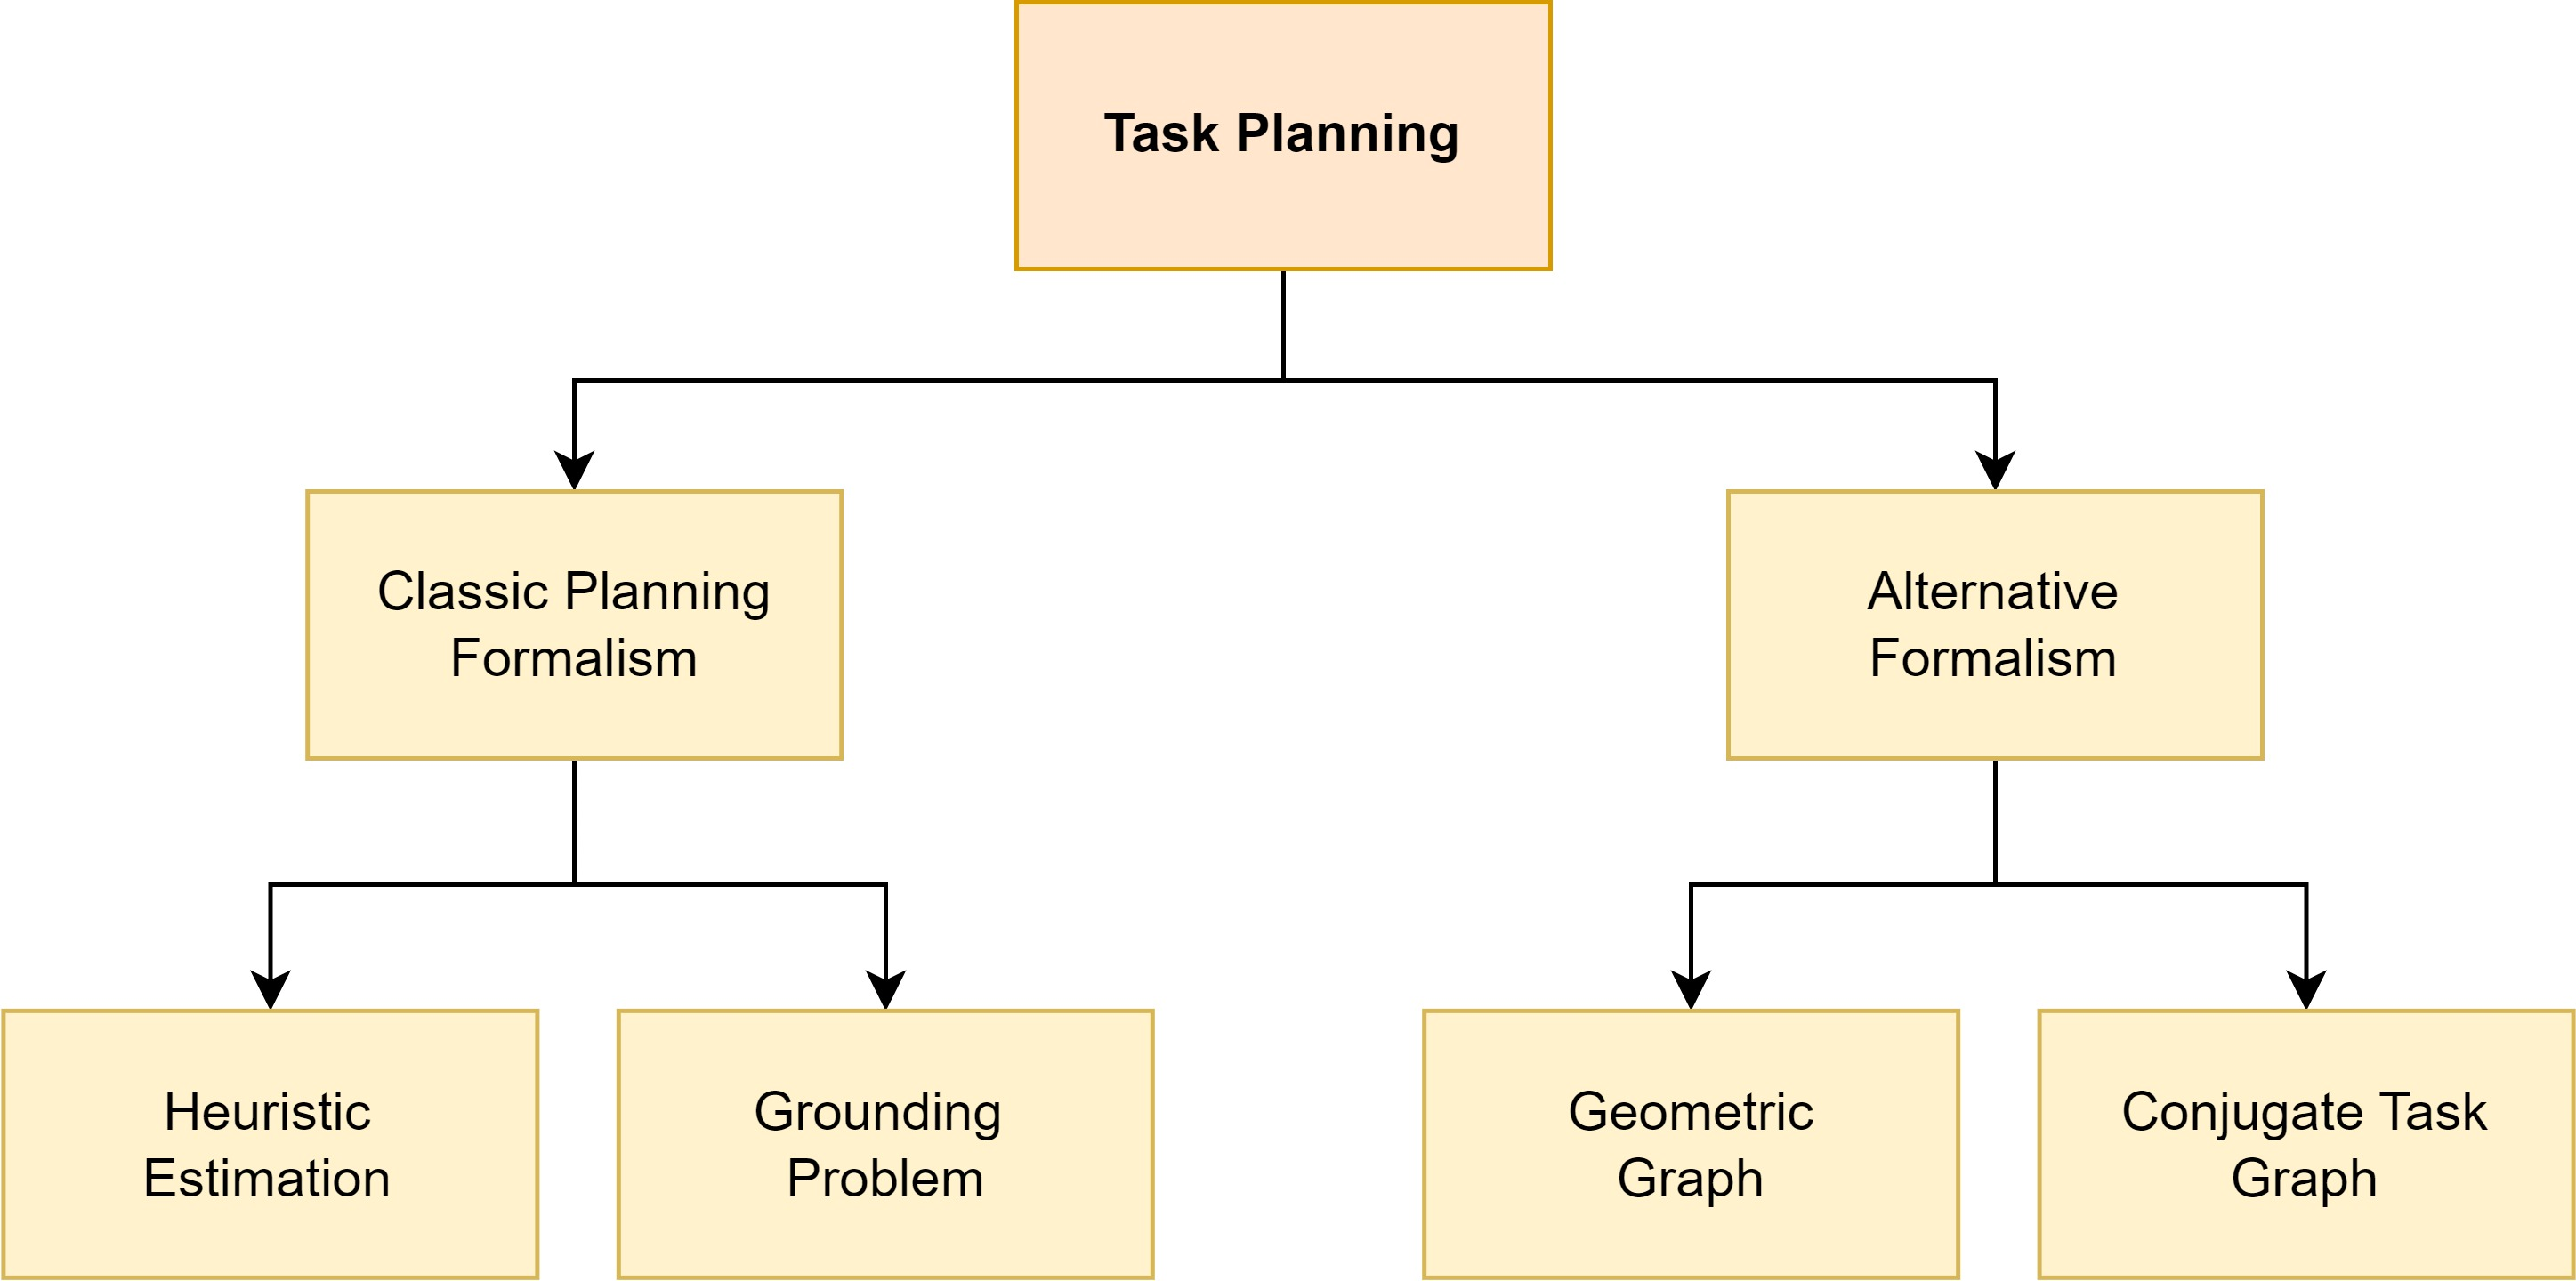
\includegraphics[width=0.8\textwidth]{figures/images/ch4/gnn_taxonomy.jpg}
    \caption{Proposed taxonomy for GNNs methods used in the context of robotic learning.}
    \label{fig:gnn_taxonomy}
\end{figure}


In general, most research has focused on solving \textit{task planning} problems. According to classical literature \cite{geffner2013concise}, a task-planning problem can be defined as a state-transition model $\Pi = \left( S, A, s_{0}, G \right)$, where $S$ is the set of states, $A$ is the set of actions, $s_{0}$ is the initial state, and $G$ is the goal state. Here, an action $a \in A$ is a function that maps a state $s \in S$ to a new state (successor) $a(s)$, i.e., $a: S \rightarrow S$. Essentially, a plan is a sequence of actions $\tau = a_{1}, a_{2}, \dots, a_{n}$ that enables the system to transition from the initial state $s_{0}$ to the goal state $s_{n} = a(s_{n-1}) = G$. Various approaches have been proposed to solve the problem of finding a plan given a specific initial and goal state. These approaches either adhere to the classical PDDL formalism \cite{aeronautiques1998pddl}, and thus fit within the traditional planning framework, or introduce novel representations that do not rely on PDDL to address the planning problem.

This review begins by examining methods that follow the \textit{Classic Planning Formalism}  (Section \ref{sec:pddl_formalism}), followed by a brief discussion of novel approaches that do not use this kind of formalism (Section \ref{sec:gnn_alternative_formalism}).

\subsection{Classic Planning Formalism}
\label{sec:pddl_formalism}
In this section, we will describe the methods that follow the classic task-planning formalism. Before introducing the methods, it is crucial to define the formalism with a set of foundational definitions.

Task-planning is a well-known problem that has been studied for many years. One of the most influent formalizations, still widely used today, is STRIPS (Stanford Research Institute Problem Solver) \cite{fikes1971strips}, which was developed in the 70s. STRIPS was initially an automated planning solver, but its primary contribution lies in its definition of a planning problem, which has served as the foundation for much of the research in subsequent decades.

According to the STRIPS formalism, a planning task is defined as a tuple $\Pi = (P, A, s_0, G, c)$, where:
\begin{itemize}
    \item $P$ is a set of propositions (also called facts).
    \item $A$ is a set of actions.
    \item A state $s$ is a subset of predicates, $s \subseteq P$, where $s_0$ is the initial state,
    \item $G \subseteq s$ represents the goal conditions.
    \item $c: A \leftarrow R$ is the cost function, which assign to an anction $a \in A$ a real-value, $c(a)$ representing the cost of performing a given action.
\end{itemize}

An action $a \in A$ is defined as a tuple $a = \left(pre(a), add(a), del(a)\right)$, where $pre(a), add(a), del(a) \subseteq P$. These represent:
\begin{itemize}
    \item $pre(a)$: the preconditions (i.e., predicates that must be true to perform the action).
    \item $add(a)$: the added conditions (i.e., predicates that become true after the action is executed).
    \item $del(a)$: the deleted conditions (i.e., predicates that become false after the action is executed).
\end{itemize}
with the constraint that $add(a) \cap del(a) = \emptyset$. According to this formalism, an action is applicable in a state $s$ if $pre(a) \subseteq s$, and it results in the successor state $s' = (s \setminus del(a)) \cup add(a)$.

Building on these foundational concepts, the \textbf{Planning Domain Definition Language} (PDDL) was introduced in the 90s \cite{aeronautiques1998pddl}. PDDL is a human-readable format for describing automated planning problems. It provides a way to describe, the possible states of the world, the set of available actions, where each action description includes the prerequisites and the effects of the action, a specific initial state of the world and a specific set of desired goals. 

PDDL separates the model of a planning problem into two main components:
\begin{enumerate}
    \item The domain description, which defines the elements that are common across all problems within a given domain.
    \item The problem description, which specifies the specific planning problem, including the initial state and the goals to be achieved.
\end{enumerate}

\begin{figure}[t]
    \centering
    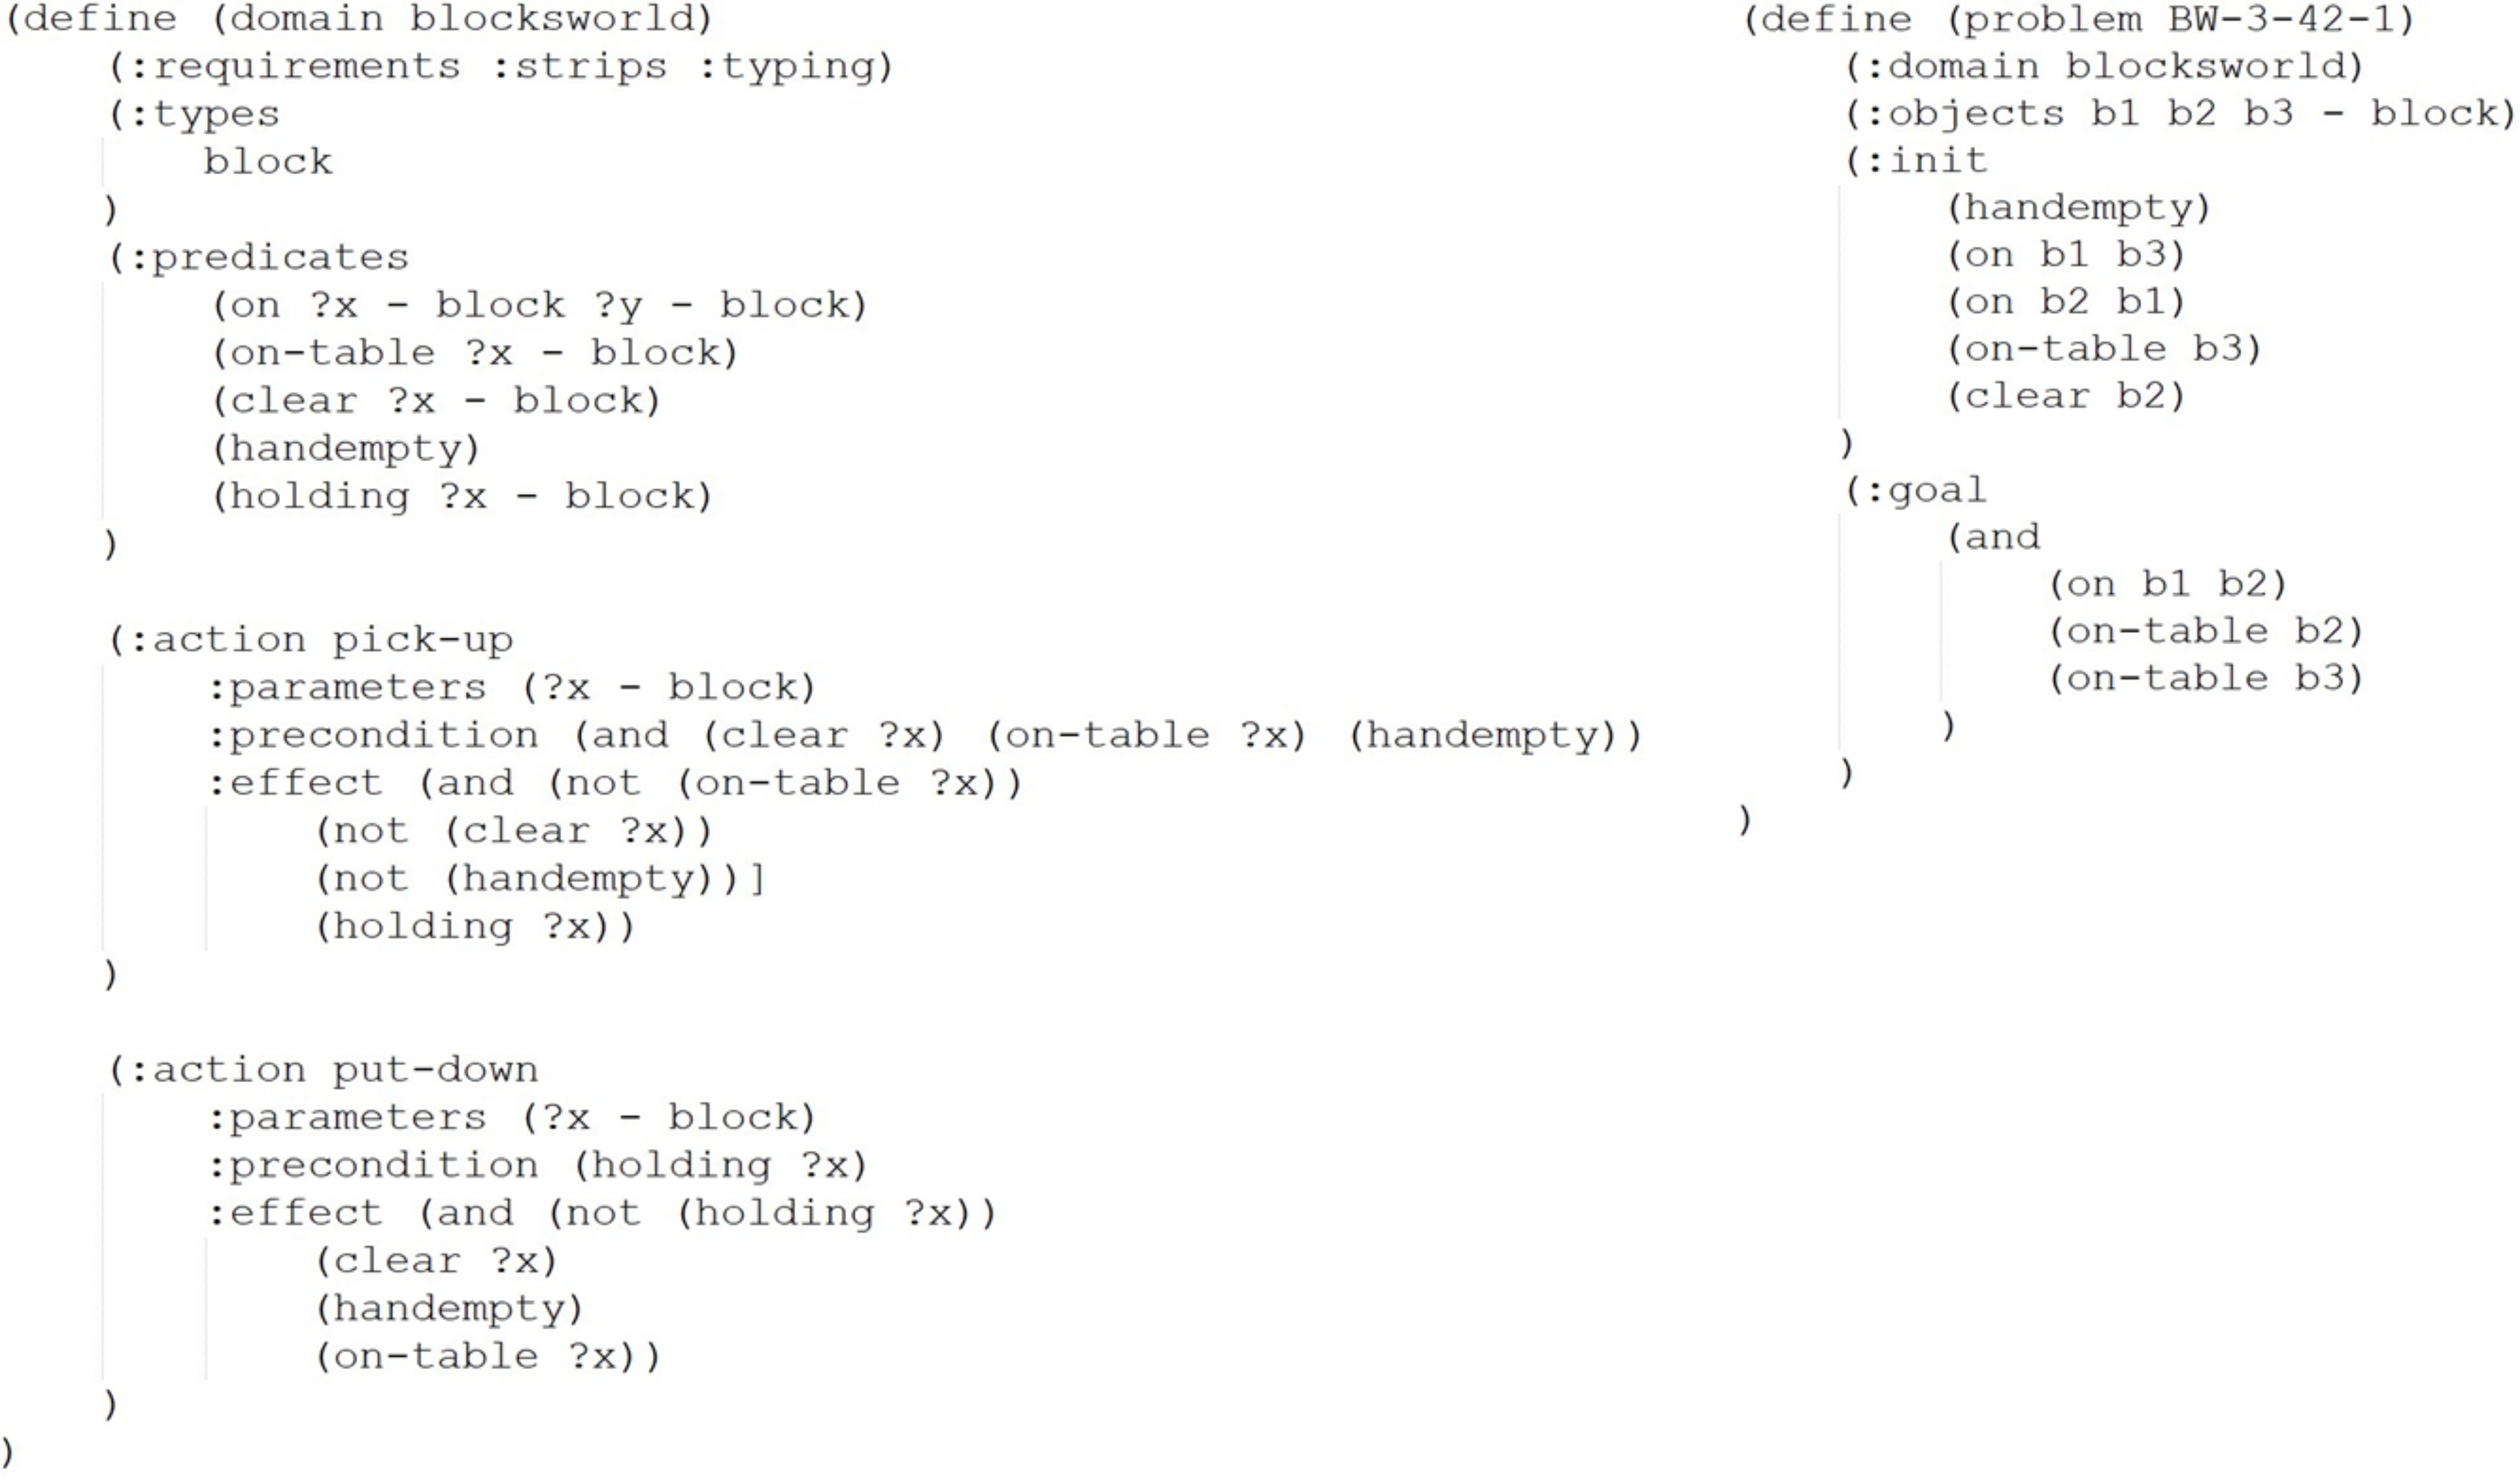
\includegraphics[width=1.0\textwidth]{figures/images/ch4/domain_problem.jpg}
    \caption{(Left) Example of a domain definition for the Blocks-World, specifying the predicates and actions available in the environment. (Right) Example of a problem definition for the domain, where a specific instance of the problem is defined, including object instances, the initial state, and the desired goal state.}
    \label{fig:domain_problem}
\end{figure}


Figure \ref{fig:domain_problem} provides examples of domain and problem definitions for the Blocks-World environment. As shown, when using the PDDL formalism, it is essential to fully define the elements of the world (e.g., blocks), the available actions (e.g., pick-up), along with their corresponding preconditions (i.e., predicates that must be true for the action to be executed) and postconditions (i.e., the effects of the actions). In the problem definition, specific instances of objects in the environment are specified, along with the initial state and goal state, both of which are defined based on the predicates available in the domain definition.

Once the problem is defined using the PDDL formalism, a complete parameterized instance must be specified to obtain a solution to the planning problem. This involves solving what is known as the \textbf{grounding problem}. During this process, all predicate and action variables must be instantiated with the objects defined in the problem. For instance, in the example shown in Figure \ref{fig:domain_problem}, the variable \( x \) is replaced with objects \( b1 \), \( b2 \), and \( b3 \) from the problem definition, leading to a complete enumeration of all predicates and actions. The result of this process is known as the \textit{Grounded Planning Problem}, which follows the same formalism as the STRIPS representation described earlier.

The grounded problem then serves as the input for planning algorithms, such as the well-known Fast Downward \cite{helmert2006fast} or LAMA \cite{richter2010lama}. While delving into the specifics of these algorithms is beyond the scope of this section, it is crucial to note that they are essentially \textit{search algorithms}. Given a state-space represented as a graph, which is derived from the Grounded STRIPS representation, these algorithms compute the (estimated) the shortest path in the state-space, connecting the source node (representing the initial state) to the target node (representing the goal state).

The limitations of these approaches have been well-known for a long time. Specifically, these algorithms do not scale well as the size of the problem (in terms of actions, predicates, and objects) increases. There are two main areas where higher problem dimensionality can cause performance issues:

\begin{enumerate}
    \item \textit{Search Phase}, as the dimensionality of the problem increases, the state-space expands correspondingly. This increases the time required to explore the state-space and find a solution path.
    \item \textit{Grounding Problem}, as the problem dimensionality grows, the time needed to generate a complete enumeration of all object combinations grows exponentially.
\end{enumerate}

To address the first issue, research has focused on developing methods to accelerate the search phase by introducing \textit{heuristics} that guide the search more efficiently towards the goal state. For the second issue, the literature has proposed methods that perform \textit{partial} grounding, concentrating on the action instances that are most relevant to the specific problem instance. Examples of these methods will be discussed in the following two paragraphs.

Here, a heuristic is a function $h: S \rightarrow \mathbb{R}$, which maps a state $s \in S$ to a real value $h(s)$, representing an estimate of the cost to reach the goal state from the state $s$. The optimal heuristic, denoted $h^{*}(s)$, is the heuristic that gives the exact cost of the optimal plan to reach a goal state from $s$. A heuristic is considered \textit{admissible} if it never overestimates the actual cost, i.e., $h(s) \leq h^{*}(s), \forall s \in S$. By utilizing the heuristic cost, a search algorithm can focus on exploring the most promising states instead of performing an exhaustive search of the entire state space.

In the context of task planning, a common heuristic is computed by solving the \textbf{Relaxed-STRIPS} problem. This is a simplified version of the STRIPS problem, where the delete conditions ($del$) are ignored, i.e., an action $a$ is represented as $a = \left(pre(a), add(a), \emptyset \right)$. The Relaxed-STRIPS problem is easier to solve because removing the $del$ conditions relaxes some of the constraints, allowing the state to include predicates that logically cannot be true simultaneously. By solving this relaxed problem, an estimated cost for reaching the goal from a given state can be computed. This approach has been used in well-known algorithms such as Fast-Downward \cite{helmert2006fast} and combined with novel heuristics in LAMA \cite{richter2010lama}.

\paragraph*{Heuristic Estimation}\mbox{}\\
In this paragraph the methods that methods that propose GNN for computing heuristics estimation through the usage of GNNs are discussed. Specifically, the review will focus on two recent works \cite{shen2020learning,chen2024learning}.

The first remarkable work towards the use of GNN for heuristic estimation was proposed by authors of \cite{shen2020learning}. Here, authors started from the idea to leverage data-driven approaches to learn an heuristic function, and explore the possibility of such methods to generalize to different cardinalities and problems, and comparing the performance of such methods with classic heuristic functions.

The first step to solve this problem is related to the definition of the input. Specifically, the authors started by the Relaxed-STRIPS formulation. The STRIPS problem can be easly formulated as a graph if the following observations are done:
\begin{itemize}
    \item A node, can be described a predicate which can be either a pre-condition or an added condition.
    \item The edge is represented by the action that connects the pre-conditions to the added-conditions. 
\end{itemize}
\smalltodo{add figure}
Figure \ref{} illustrates the mapping of predicates and actions to graph nodes and edges. As can be observed, an action connects multiple nodes. To model this, the authors use a generalized graph structure known as a \textit{hypergraph}. Formally, a hypergraph is defined as a triple $G = (u, V, E)$, where $V = \left\{ \textbf{v}_{i}: i \in \left\{1, 2, \dots, N^{v} \right\} \right\}$ is the set of $N^{v}$ vertices, and $E = \left\{ (e_{k}, R_{k}, S_{k}): k \in \left\{1, 2, \dots, N^{e} \right\} \right\}$ is the set of $N^{e}$ hyper-edges. In this structure, $R_{k}$ is the receiver set, containing the indices of the nodes for which the $k$-th edge acts as an incoming edge, and $S_{k}$ is the sender set, containing the indices of the nodes for which the $k$-th edge acts as an outgoing edge. Then, $\textbf{v}_{i}$ is the node embedding, which has been implemented as a binary-vector $v_i = [x_s, x_g]$, where $x_s, x_g \in \left\{0,1\right\}$. $x_s=1$ iff the i-th predicate is true in the state s and $x_g=1$ iff the predicate is true in the goal-state. While, $e_{k}$ is the edge embedding, $e_k = [c(a_k), |Pre(a_k)|, |Add(a_k)|]$, where $c(a_k)$ is the cost of the operator, $|Pre(a_k)|$ is the number of pre-condition and $|Add(a_k)|$ is the number of added condition.

Once the graph structure has been defined, the module that processes this input can be described. Specifically, the authors propose leveraging the concept behind the \textit{Interaction Network} \cite{battaglia2016interaction}. The architecture, depicted in Figure \ref{}, implements the computational flow shown in Figure \ref{}, and can be divided into the following three steps.

\begin{enumerate}
    \item The \textit{Encoding Block} consists of two functions, $\phi^{e}$ and $\phi^{v}$, both implemented as Multi-Layer Perceptrons (MLPs). These functions transform the initial binary inputs into higher-dimensional representations, specifically, $\phi^{e}(e_j)$ produces $e_{hid}^{0}$ and $\phi^{v}(v_i)$ produces $v_{hid}^{0}$, where both $e_{hid}^{0}$ and $v_{hid}^{0} \in \mathbb{R}^{32}$. This step expands the original binary vectors (of size 2 or 3) into 32-dimensional vectors.

    \item The \textit{Core Block} implements the Message-Passing Iterative Procedure and is divided into the following steps:

        \begin{enumerate}
            \item \textit{Edge Block}: For each edge (representing an action), $e_{hid,j}^{t-1}$ is generated by concatenating the embeddings of the receiver and sender nodes associated with the edge. An MLP encoder is then applied to this concatenated information to create a new edge representation $e_{hid,j}^{t}$.

            \item \textit{Node Block}: Similar to the Interaction Network, only the receiver nodes' states are updated. The edge information influencing each receiver is aggregated by summing the embeddings of the incoming edges using the function $\rho^{e \rightarrow v}$. The node input is constructed by concatenating the incoming edge embeddings $e_{hid,j}^{t}$, the initial node embedding $v_{hid,i}^{0}$, and the previous node state $v_{hid,i}^{t-1}$. This concatenated input is then passed through an MLP to generate the updated node representation $v_{hid,i}^{t}$.

            \item \textit{Global Block}: This block updates the global graph representation by aggregating both node and edge embeddings using the functions $\rho^{e \rightarrow u}$ and $\rho^{v \rightarrow u}$, respectively. The aggregated information is passed through an MLP to produce the new global graph representation.
        \end{enumerate}

    \item The \textit{Decoding Block} acts as a decoder, implemented as an MLP. It takes the updated global graph representation as input and generates a heuristic value for a given state, aiding in the decision-making process.
\end{enumerate}

The operations in the core block are repeated for $M$ iterations, where $M = 10$ in this work.
The system is trained by minimizing the loss function defined in Equation \ref{equation:loss_func}. Here, $h^{*}(s)$ represents the ground truth heuristic value for state $s$, obtained by solving the training planning problem with a classical planning algorithm.
\begin{equation}
    \mathcal{L}_\theta(\mathcal{B})=\frac{1}{|\mathcal{B}|} \sum_{\left(G, h^*(s)\right) \in \mathcal{B}} \frac{1}{M} \sum_{t \in \{1, \ldots, M\}}\left(h_t^\theta(G)-h^*(s)\right)^2
    \label{equation:loss_func}
\end{equation}

Interesting results were obtained during the experiments. Notably, the system demonstrated the ability to learn both domain-dependent heuristics (when tested on the same domain it was trained on) and domain-independent heuristics (when tested on a different domain). This shows that the trained GNN was capable of generating meaningful heuristic values that could be effectively used by search algorithms like A*. However, a general drawback of this approach is the time required to compute the heuristic, particularly when the model is run on a CPU instead of a GPU, which significantly impacts performance.

Development of such work was proposed by \cite{chen2024learning},
\smalltodo{ToContinue}

\paragraph*{Grounding Problem}\mbox{}\\
As stated before, one of the preliminary problem to solve, before running the search algorithm, is the Grounding Problem. In this problem 
\smalltodo{ToContinue}
\subsection{Alternative Formalism}
\label{sec:gnn_alternative_formalism}

This section discusses methods that do not rely on classical planning but instead use a graph-based environment representation, where nodes represent objects and edges denote relationships or possible actions. This structure allows Graph Neural Networks to process the graph and select the next high-level action for the robot. The following paragraphs explore different environment representations and how the network's output is translated into robot actions.

\paragraph*{Geometric Graph} \mbox{}\\
This section explores methods based on the concept of the Geometric Graph. In its initial formulation \cite{lin2022efficient}, a Geometric Graph is a scene representation where nodes correspond to task-relevant entities, such as objects and their target positions. A fully connected graph is constructed by linking two types of nodes: \textit{object} nodes, which represent current instances of objects with their positions as attributes, and \textit{goal} nodes, which represent the desired final positions of these objects, also characterized by spatial attributes.

Using this representation, a GNN can be trained to perform node classification. At each step, an object node and a goal node are selected, representing the object to move and its target position. With these selections, a pick-and-place primitive can be executed. An example of this inference process is shown in Figure \ref{fig:geometric_graph_computation}.
\begin{figure}[t]
    \centering
    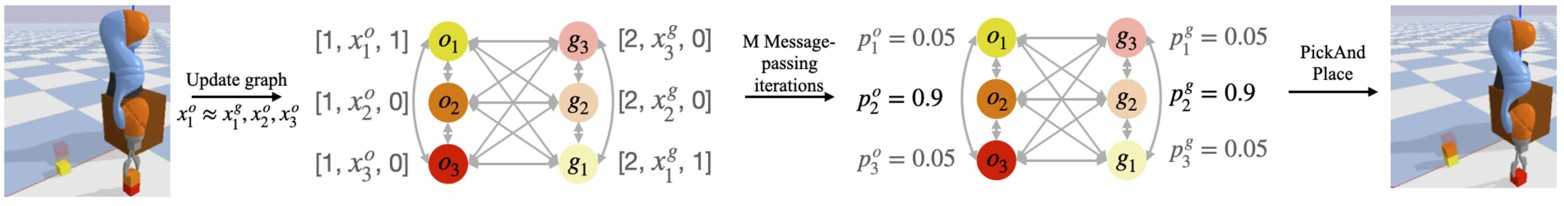
\includegraphics[width=1\textwidth]{figures/images/ch4/geometric_graph_computation.jpg}
    \caption{Computation flow in a scene represented by a Geometric Graph. Object nodes ($o_{i}$) and goal nodes ($g_{i}$) are created, with edges connecting them based on spatial and semantic relationships. A GNN classifies the nodes, selecting one object node and one goal node. These nodes are then passed as input to a motion primitive, which generates the necessary actions to move the selected object towards the target goal.}
    \label{fig:geometric_graph_computation}
\end{figure}

% \smalltodo{add figure}

A similar approach is presented in \cite{di2023one}, where two GNNs are trained separately to classify an object node and a goal node.

While these methods are noteworthy because they can solve multi-step tasks through supervised learning without relying on a planning algorithm, they have significant limitations. The most notable is their dependency on knowing both the current and target positions of the objects. In these early studies, such information is provided either by the simulation environment or by using special markers on objects in real-world settings to facilitate position estimation.

To address these limitations, the authors in \cite{zhu2021hierarchical} extended the Geometric Graph concept and proposed a new representation called the \textit{Symbolic Scene Graph}. In this framework, a 3D Object Pose Estimation module is used to extract objects from the scene, constructing a geometric graph. Edges are then added based on predefined relationships (e.g., ``can1 on shelf A", as illustrated in Figure \ref{fig:geometric_scene_graph}). The next step in the planning process is determined using a Neuro-Symbolic Task Planning module \cite{xu2019regression}, which takes the current Symbolic Scene Graph and the goal (expressed as desired predicates, i.e., relationships between objects) as input. This module outputs the next action, expressed as a subgoal achievable with a single motion primitive.
\begin{figure}[t]
    \centering
    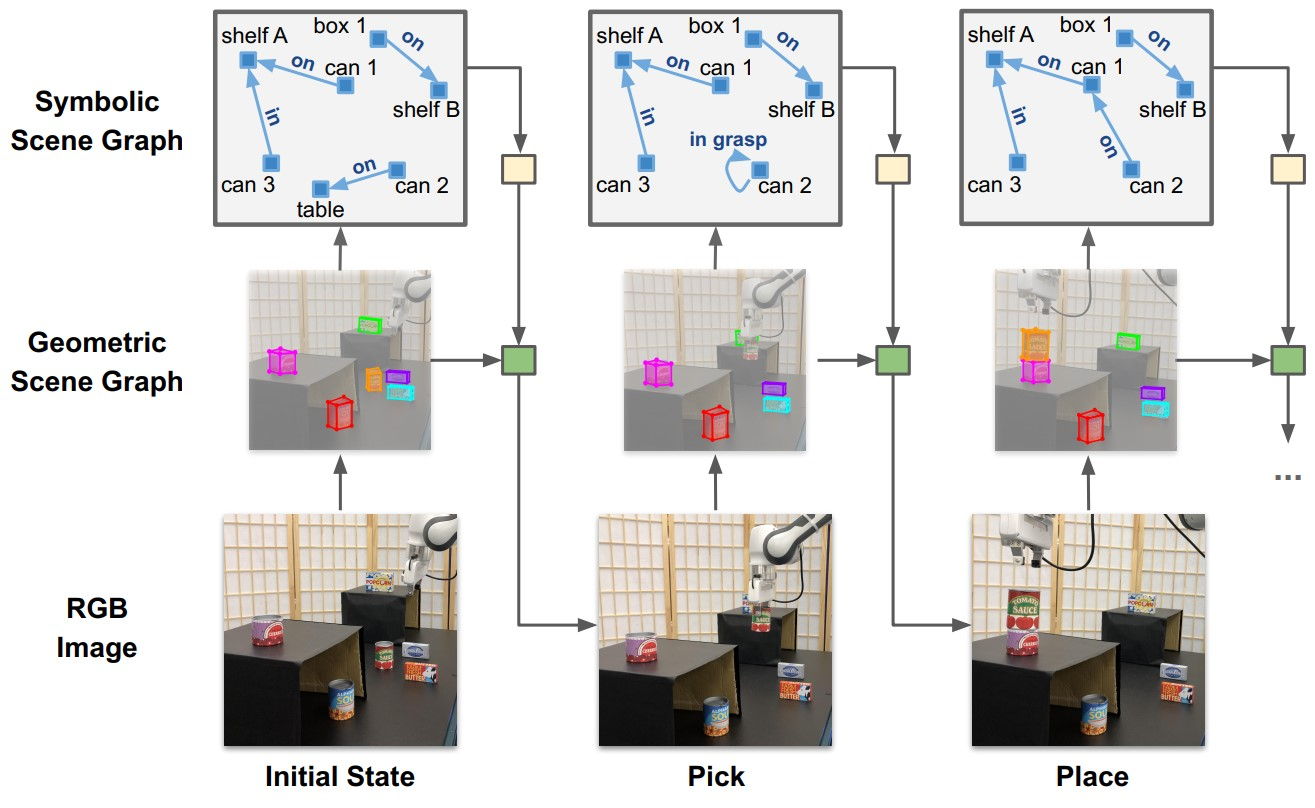
\includegraphics[width=0.8\textwidth]{figures/images/ch4/geometric_scene_graph.jpg}
    \caption{Example of a Symbolic Scene Graph. The graph is constructed by extracting objects from the scene and adding edges based on predefined relationships.}
    \label{fig:geometric_scene_graph}
\end{figure}


While this method showed promising results, including reduced computation times compared to the PDDLStream \cite{garrett2020pddlstream} baseline, it has limitations. The primary challenge lies in the cognitive module, which relies on 3D object pose estimation. This technique is only robust and reliable when used with pre-known objects.

\paragraph*{Conjugate Task Graph} \mbox{}\\
The Conjugate Task Graph (CTG) \cite{huang2019neural} addresses challenges in constructing traditional Task Graphs, where nodes represent states and edges represent transitions. For novel tasks, mapping states to new nodes is often infeasible. In contrast, the CTG uses nodes to represent actions, with edges implicitly representing states and their preconditions (Figure \ref{fig:conjugate_task_graph}).
\begin{figure}[t]
    \centering
    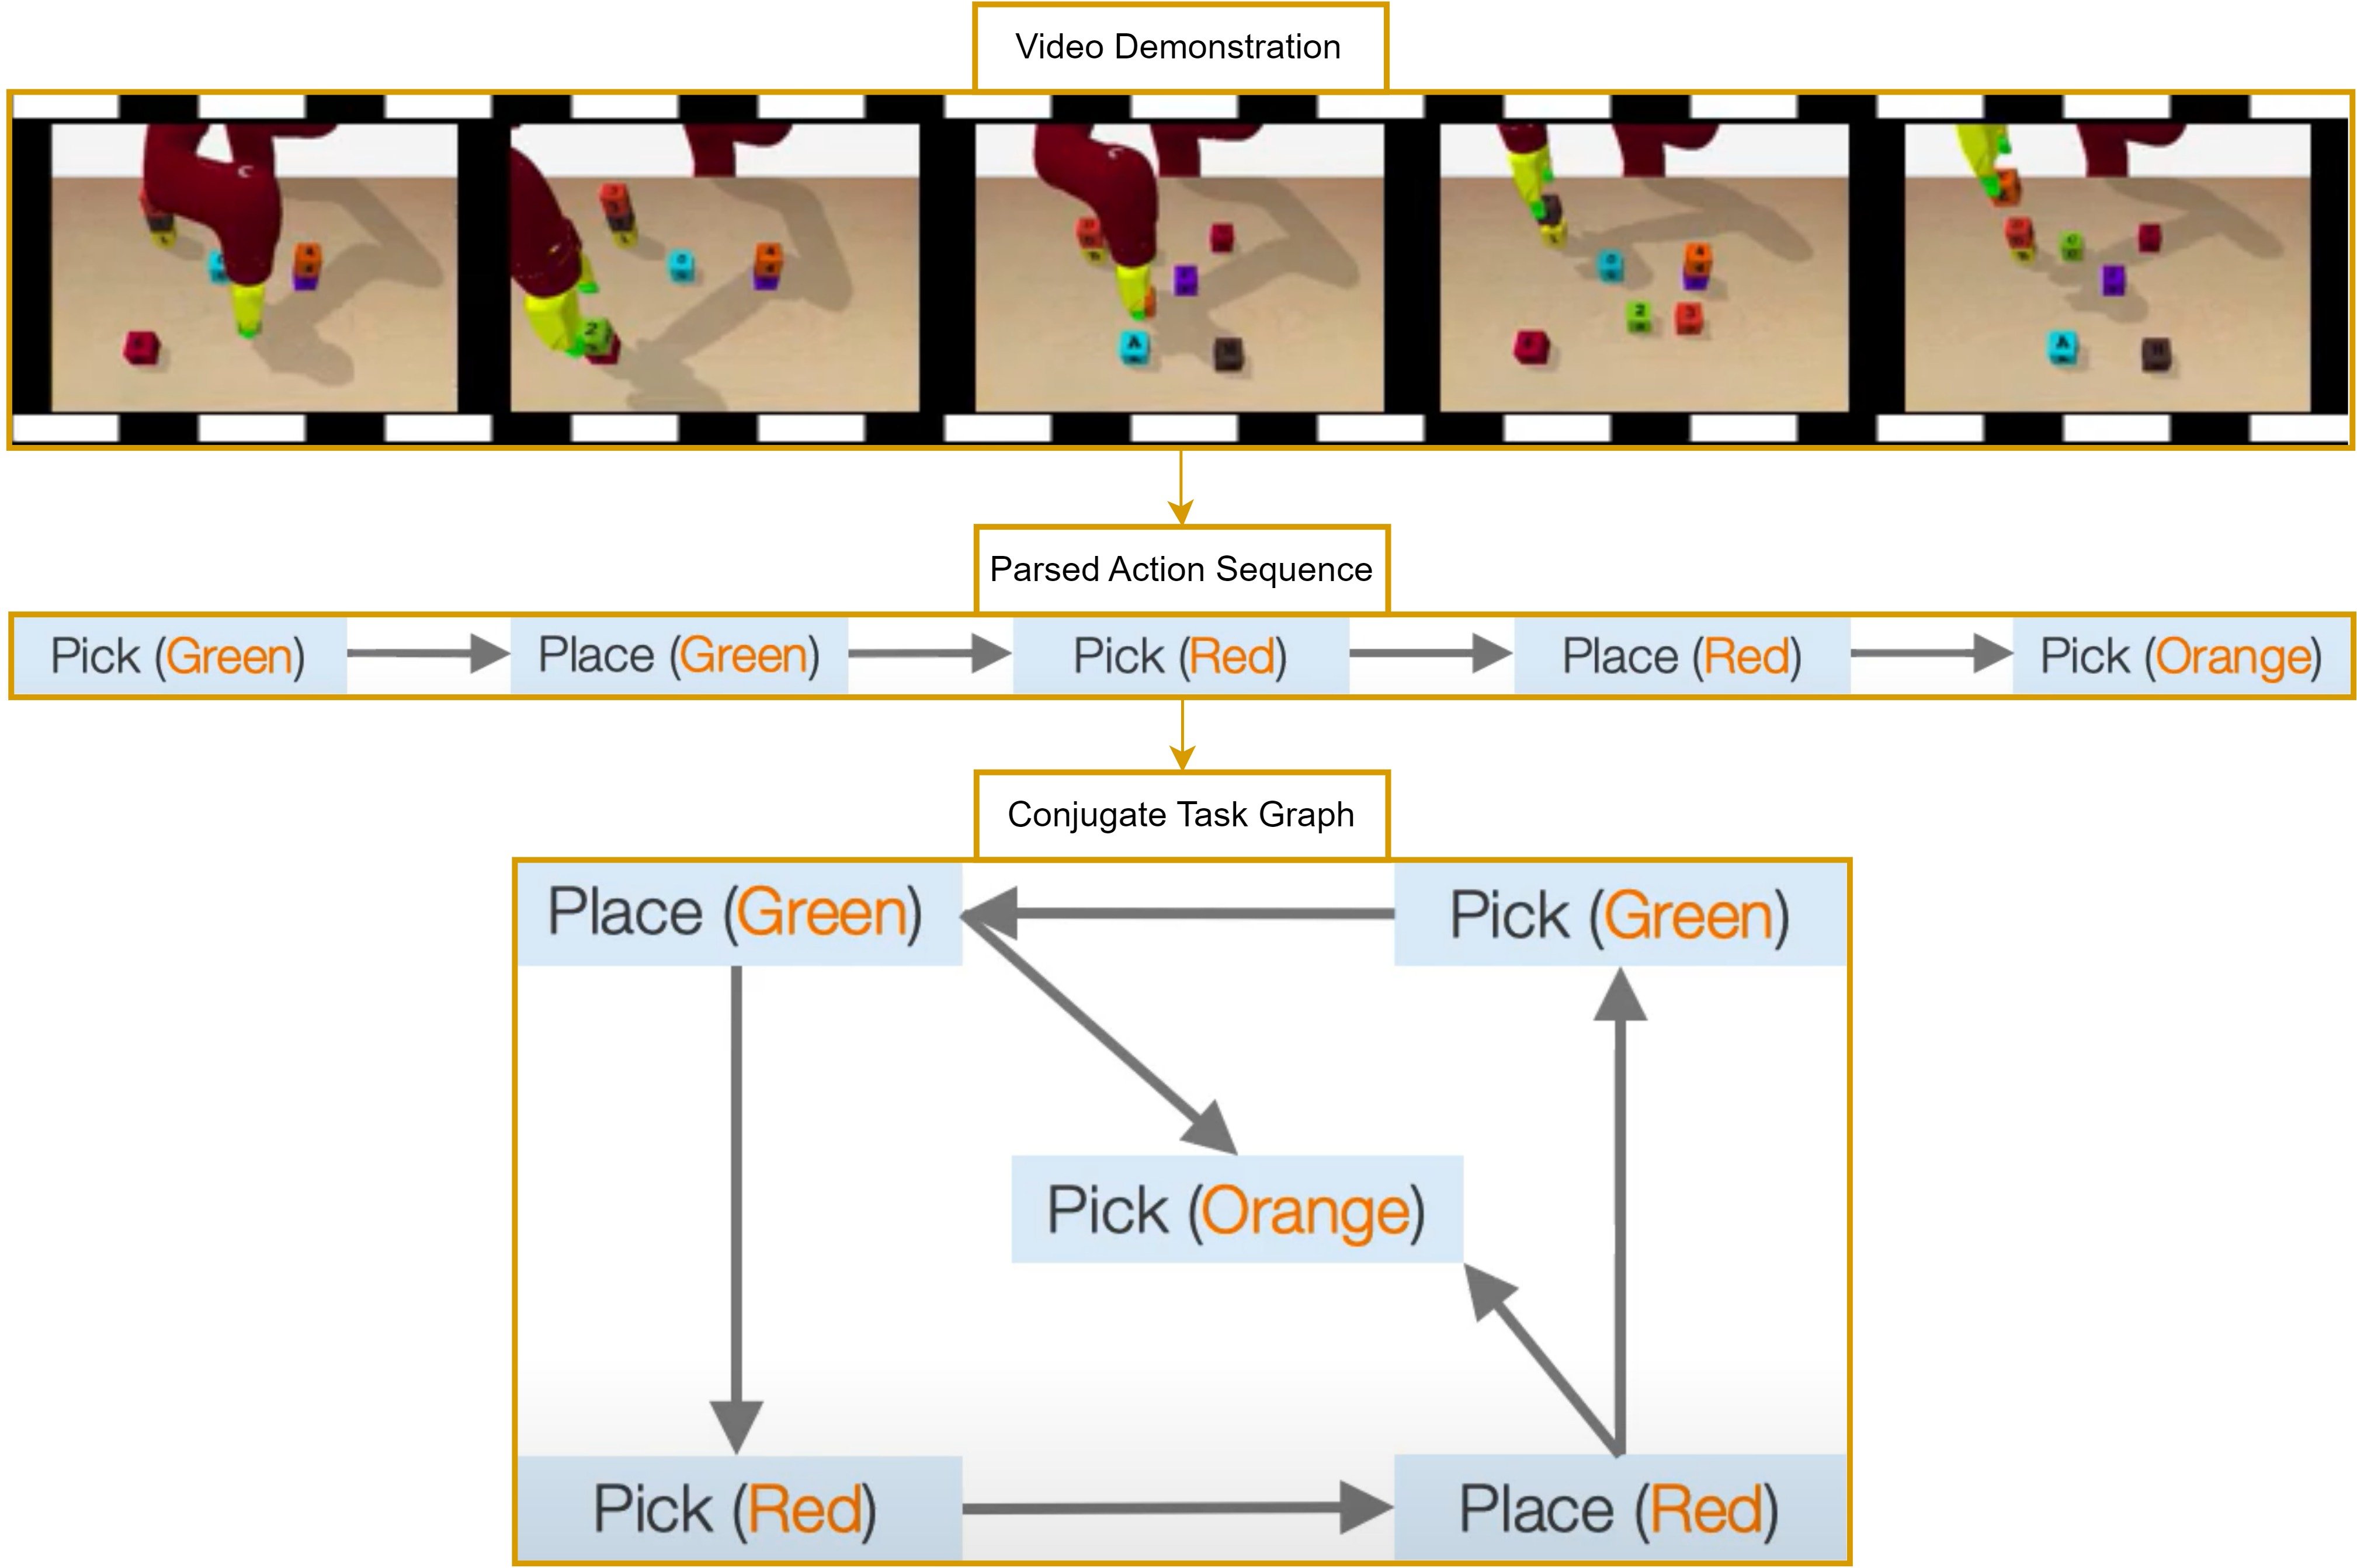
\includegraphics[width=0.8\textwidth]{figures/images/ch4/conjugate_task_graph.jpg}
    \caption{Conjugate Task Graph representation. Starting from the video demonstration, the sequence of actions is extracted and used to construct the initial graph. Then the complete Conjugate Task Graph is built by predicting the missing edges, which represents possible actions sequences observed in the training set.}
    \label{fig:conjugate_task_graph}
\end{figure}

Based on this representation, and assuming all possible actions have been observed in the training set, it is possible to build and train a modular architecture composed of the following components:
\begin{itemize}
    \item \textit{Demo Interpreter}: A Convolutional Neural Network \\ trained to extract the sequence of actions performed by a robot from a given demonstration. This sequence of actions is used to construct an initial graph.
    
    \item \textit{Graph Completion}: A Graph Neural Network trained to complete the graph produced by the Demo Interpreter. This module predicts the missing edges in the graph, representing unseen transitions between actions.
    
    \item \textit{Node Localization}: A Multi-Layer Perceptron that, given the current observation's encoding and the embeddings of the nodes in the graph, predicts the node corresponding to the action the robot is currently performing.
    
    \item \textit{Edge Localization}: Another MLP that, given the current observation's encoding and the node embeddings, predicts the edge representing the next transition and, consequently, the next action the robot should take.
\end{itemize}

The complete architecture was trained end-to-end, and experimental results demonstrate its effectiveness in multi-step tasks, such as object ordering and stacking. The CTG representation enables the policy to generalize to novel sequences of actions, making it particularly well-suited for tasks like object ordering.

However, this approach fails to generate valid paths when the demonstration includes out-of-distribution observations, produced by sequences of actions that were never encountered in the training set. Additionally, experimental results reveal that this method struggles to perform tasks requiring more than 6 steps. This limitation arises mainly from the Demo Interpreter module, which must generate long action sequences to instantiate the CTG.


In conclusion, with respect to the discussed method, the goal of this chapter is to evaluate and assess the feasibility of using data-driven methods for heuristic estimation within a specific domain of interest. This evaluation aims to explore the potential of leveraging such methods in \textbf{future works}, where integrating low-level policies within high-level planning tasks could enable generalization to multi-step tasks.

\section{Experimental Results}
\label{sec:gnn_experimental_results}
In this section, the experimental results are presented. These results are preliminary within the context of this thesis and primarily aim to evaluate the performance and limitations of using GNNs for learning heuristics, specifically through the assessment of the STRIPS-HGN method proposed in \cite{shen2020learning}.

The method was tested in the well-known \textit{BlockWorld} domain \cite{slaney2001blocks}. This domain consists of a single object type, the \textbf{block}. 
This domain then, contains five predicates, and four actions that are listed below: 

\begin{itemize}
    \item \textit{On}: True if block $x$ is on block $y$.
    \item \textit{On-Table}: True if block $x$ is on the table.
    \item \textit{Clear}: True if block $x$ has no object on top, making it available for manipulation.
    \item \textit{Handempty}: True if the robotic gripper is not holding any object.
    \item \textit{Holding}: True if the robotic gripper is holding block $x$.

    \item \textit{Pick-Up}: Picks up block $x$ if it is clear, on the table, and the gripper is empty.
    \item \textit{Put-Down}: Places the block currently held by the gripper onto the table.
    \item \textit{Stack}: Stacks block $x$ (held by the gripper) onto a clear block $y$.
    \item \textit{Unstack}: Removes block $x$ from on top of block $y$ (if block $x$ is clear) and picks it up with the gripper.
\end{itemize}

For the experiments, 50 problem instances of varying complexity were generated, with complexity measured by the number of blocks, ranging from 3 to 15. The STRIPS-HGN was trained on a subset of problems with block counts between 5 and 10. Testing was conducted in two scenarios:

\begin{itemize}
    \item \textit{In-Training Distribution}: The model was tested on new problems with complexities within the same range as the training data.
    \item \textit{Out-of-Training Distribution}: The model was tested on problems with unseen complexities (3, 4, 11, 12, 13, and 15 blocks).
\end{itemize}

The ground-truth heuristic ($h^{*}$) was computed by solving each problem instance using the Scorpion planning solver \cite{seipp2020saturated}, in a configuration that ensure the optimality of the solution. In this case, the heuristic is represented as the number of actions needed to reach the goal state from the initial state.
% configured with the LAMA search algorithm \cite{richter2010lama}. While this setup does not guarantee path optimality, it provides the most reliable method for obtaining a solution across all 50 problem instances, regardless of task complexity, within a 16-minute time limit per instance.

The STRIPS-HGN performance was compared against several classic heuristics, including:
$h_{max}$, an admissible heuristic; $h_{add}$, a generally faster heuristic; $LM-cut$ \cite{richter2010lama}, a heuristic offering a balance between path optimality and speed. The STRIPS-HGN was also compared against itself with different numbers of planning steps (1, 5, and 10).

Moreover, different metrics have been proposed to compare the different algorithms. Specifically, the algorithms are compared with respect to:
\begin{itemize}
    \item \textit{Number of expanded nodes}, this measures the number of nodes that are traversed during the exploration of the state-space in order to find a given solution. This number is accumulated over the different problems of a given complexity, then the average and standard deviation is computed.
    \item \textit{Search time}, this measures the time needed for the algorithm to return a valid solution.  This number is accumulated over the different problems of a given complexity, then the average and standard deviation is computed.
    \item \textit{Plan length}, this measures the number of actions that are needed to reach a solution. This number is accumulated over the different problems of a given complexity, then the average and standard deviation is computed.
    \item \textit{Ratio of solution found}, this measures the ratio of number of times the search algorithm with a given heuristic returns a solution before a timeout of 5 minutes over all the number of problems.
\end{itemize}

\paragraph*{In-Training Distribution Generalization}\mbox{}\\
The first generalization test performed was related to the In-Training Distribution Generalization. This means that the algorithms are tested on 10 novel problem instances for each problem complexity.
The first results are related to the number of solution found, reported in Table \ref{table:in_distribution_cnt_success}. It can be noted how most of the heuristics are able to completely return a solution in the given timeout. This does not happen for the admissible heuristic $h_{max}$, which starts to not return a valid solution, starting from the complexity of 9 boxes. 

\begin{table}[t]
    \centering
    % \refstepcounter{table}
    \caption{Comparison of ``ratio of solution found'' on BlocksWorld domain across different complexities (Comp.). The table presents the results for $h_{max}$, $h_{add}$, $LM-cut$, and Strips-HGN with 1, 5, and 10 steps.}
    \label{table:in_distribution_cnt_success}
    \resizebox{\linewidth}{!}{%
    \begin{tabular}{|c|c|c|c|c|c|c|} 
    \hline
    \textbf{Comp.} & $\mathbf{h_{max}}$ & $\mathbf{h_{add}}$ & $\mathbf{LM-cut}$ & $\mathbf{Strips-HGN_1}$ & $\mathbf{Strips-HGN_5}$ & $\mathbf{Strips-HGN_{10}}$ \\ 
    \hhline{|=======|}
    5 & 1.00 & 1.00 & 1.00 & 1.00 & 1.00 & 1.00 \\ 
    \hline
    6 & 1.00 & 1.00 & 1.00 & 1.00 & 1.00 & 1.00 \\ 
    \hline
    7 & 1.00 & 1.00 & 1.00 & 1.00 & 1.00 & 1.00 \\ 
    \hline
    8 & 1.00 & 1.00 & 1.00 & 1.00 & 1.00 & 1.00 \\ 
    \hline
    9 & 0.00 & 1.00 & 1.00 & 1.00 & 1.00 & 1.00 \\ 
    \hline
    10 & 0.10 & 1.00 & 0.9 & 1.00 & 1.00 & 1.00 \\
    \hline
    \end{tabular}
    }
    \end{table}

To provide more insight into the generalization capabilities of STRIPS-HGN with respect to the training distribution, Tables \ref{table:in_distribution_avg_nodes_expanded}, \ref{table:in_distribution_avg_search_time}, and \ref{table:in_distribution_avg_plan_length} report key metrics, including the number of expanded nodes, search time, and plan length, respectively.

\begin{landscape}
\begin{table}
    \centering
    \caption{Mean and standard deviation of ``number of expanded nodes'' on the BlocksWorld domain across different complexities (Comp.). The table presents the results for $h_{max}$, $h_{add}$, $LM-cut$, and Strips-HGN with 1, 5, and 10 steps.}
    \label{table:in_distribution_avg_nodes_expanded}
    \resizebox{\linewidth}{!}{%
    \begin{tabular}{|c|c|c|c|c|c|c|} 
    \hline
    \textbf{Comp.} & $\mathbf{h_{max}}$ & $\mathbf{h_{add}}$ & \begin{tabular}[c]{@{}c@{}}\textbf{LM-}\textbf{cut}\end{tabular} & \begin{tabular}[c]{@{}c@{}}\textbf{Strips-}\textbf{HGN\textsubscript{1}}\end{tabular} & \begin{tabular}[c]{@{}c@{}}\textbf{Strips-}\textbf{HGN\textsubscript{5}}\end{tabular} & \begin{tabular}[c]{@{}c@{}}\textbf{Strips-}\textbf{HGN\textsubscript{10}}\end{tabular} \\
    \hhline{|=======|}
    5 & $98.80 \pm 97.06$ & $22.00 \pm 14.68$ & $24.40 \pm 23.30$ & $16.50 \pm 10.31$ & $\mathbf{12.40 \pm 3.29}$ & $12.90 \pm 3.70$ \\ 
    \hline
    6 & $643.70 \pm 430.89$ & $38.70 \pm 22.12$ & $35.10 \pm 22.56$ & $17.50 \pm 5.16$ & $\mathbf{17.10 \pm 6.77}$ & $17.30 \pm 6.42$ \\ 
    \hline
    7 & $3918.80 \pm 3124.33$ & $54.40 \pm 23.86$ & $83.70 \pm 100.14$ & $29.80 \pm 15.96$ & $27.90 \pm 12.29$ & $\mathbf{27.90 \pm 12.19}$ \\ 
    \hline
    8 & $77988.50 \pm 53611.24$ & $142.70 \pm 64.76$ & $481.60 \pm 558.93$ & $\mathbf{109.90 \pm 98.16}$ & $126.40 \pm 100.73$ & $119.90 \pm 94.02$ \\ 
    \hline
    9 & $154351.20 \pm 3673.33$ & $307.70 \pm 176.77$ & $758.90 \pm 1073.05$ & $99.70 \pm 94.47$ & $\mathbf{44.00 \pm 20.83}$ & $47.30 \pm 24.00$ \\ 
    \hline
    10 & $103801.70 \pm 11155.55$ & $366.20 \pm 320.12$ & $2799.70 \pm 4595.73$ & $235.90 \pm 270.38$ & $150.80 \pm 229.64$ & $\mathbf{95.70 \pm 110.71}$ \\
    \hline
    \end{tabular}
    }
    \end{table}
\end{landscape}
\begin{table}[t]
    \centering
    \caption{Mean and standard deviation of ``search time''  on the BlocksWorld domain across different complexities. The table presents the results for $h_{max}$, $h_{add}$, $LM-cut$, and Strips-HGN with 1, 5, and 10 steps.}
    \label{table:in_distribution_avg_search_time}
    \resizebox{\linewidth}{!}{%
    \begin{tabular}{|c|c|c|c|c|c|c|} 
    \hline
    \textbf{Complexity} & $\mathbf{h_{max}}$ & $\mathbf{h_{add}}$ & $\mathbf{LM-cut}$ & $\mathbf{Strips-HGN_1}$ & $\mathbf{Strips-HGN_5}$ & $\mathbf{Strips-HGN_{10}}$ \\ 
    \hhline{|=======|}
    5 & $0.05 \pm 0.05$ & $\mathbf{0.01 \pm 0.01}$ & $0.05 \pm 0.06$ & $0.13 \pm 0.08$ & $0.31 \pm 0.10$ & $0.57 \pm 0.20$ \\ 
    \hline
    6 & $0.53 \pm 0.31$ & $\mathbf{0.04 \pm 0.02}$ & $0.18 \pm 0.13$ & $0.20 \pm 0.07$ & $0.56 \pm 0.24$ & $1.05 \pm 0.41$ \\ 
    \hline
    7 & $4.10 \pm 2.99$ & $\mathbf{0.08 \pm 0.03}$ & $0.58 \pm 0.62$ & $0.36 \pm 0.18$ & $1.04 \pm 0.55$ & $1.74 \pm 0.97$ \\ 
    \hline
    8 & $95.44 \pm 53.45$ & $\mathbf{0.34 \pm 0.19}$ & $5.94 \pm 6.98$ & $1.68 \pm 1.55$ & $5.52 \pm 4.60$ & $9.73 \pm 8.03$ \\ 
    \hline
    9 & $300.00 \pm 0.00$ & $\mathbf{0.88 \pm 0.47}$ & $13.10 \pm 18.61$ & $1.79 \pm 1.44$ & $2.10 \pm 1.06$ & $4.11 \pm 2.28$ \\ 
    \hline
    10 & $289.29 \pm 32.15$ & $\mathbf{1.44 \pm 1.14}$ & $69.89 \pm 114.03$ & $4.79 \pm 5.35$ & $8.90 \pm 13.89$ & $11.05 \pm 14.90$ \\
    \hline
    \end{tabular}
    }
    \end{table}
\begin{table}[t]
    \centering
    \caption{Mean and standard deviation of ``plan length'' on the BlocksWorld domain across different complexities. The table presents the results for $h_{max}$, $h_{add}$, $LM-cut$, and Strips-HGN with 1, 5, and 10 steps.}
    \label{table:in_distribution_avg_plan_length}
    \resizebox{\linewidth}{!}{%
    \begin{tabular}{|c|c|c|c|c|c|c|} 
    \hline
    \textbf{Complexity} & $\mathbf{h_{max}}$ & $\mathbf{h_{add}}$ & $\mathbf{LM-cut}$ & $\mathbf{Strips-HGN_1}$ & $\mathbf{Strips-HGN_5}$ & $\mathbf{Strips-HGN_{10}}$ \\ 
    \hhline{|=======|}
    5 & $10.20 \pm 2.09$ & $10.60 \pm 2.69$ & $10.20 \pm 2.09$ & $10.20 \pm 2.09$ & $10.20 \pm 2.09$ & $10.20 \pm 2.09$ \\ 
    \hline
    6 & $13.00 \pm 2.72$ & $14.80 \pm 3.25$ & $13.00 \pm 2.72$ & $13.00 \pm 2.72$ & $13.00 \pm 2.72$ & $13.00 \pm 2.72$ \\ 
    \hline
    7 & $15.40 \pm 2.69$ & $16.60 \pm 2.97$ & $15.40 \pm 2.69$ & $15.40 \pm 2.69$ & $15.40 \pm 2.69$ & $15.40 \pm 2.69$ \\ 
    \hline
    8 & $18.80 \pm 2.23$ & $20.60 \pm 3.10$ & $18.80 \pm 2.23$ & $18.80 \pm 2.23$ & $18.80 \pm 2.23$ & $18.80 \pm 2.23$ \\ 
    \hline
    9 & - & $26.00 \pm 3.69$ & $23.00 \pm 2.72$ & $23.00 \pm 2.72$ & $23.00 \pm 2.72$ & $23.00 \pm 2.72$ \\ 
    \hline
    10 & - & $26.40 \pm 3.67$ & $23.11 \pm 3.14$ & $23.60 \pm 3.32$ & $23.40 \pm 3.10$ & $23.40 \pm 3.10$ \\
    \hline
    \end{tabular}
    }
    \end{table}

The results indicate that STRIPS-HGN can generate a valid path while using a limited number of nodes compared to traditional heuristics. This advantage is particularly pronounced at the complexity of 10 boxes, where $STRIPS-HGN_{10}$ requires an average of only 95.70 nodes to produce a valid path. This represents a significant improvement over other heuristics, which typically need a greater number of nodes to achieve similar results.

Regarding search time, it is noteworthy that $STRIPS-HGN_1$, starting from complexity 7, generates valid paths in less time than the admissible heuristic $h_{max}$ and the well-known trade-off heuristic $LM-cut$. The only heuristic that outperforms STRIPS-HGN in terms of speed is the $h_{add}$ heuristic, recognized for its faster performance relative to the others. However, this speed comes at a cost: all STRIPS-HGN variants produce paths that are shorter on average compared to those generated by the $h_{add}$ heuristic.


\paragraph*{Out-of-Training Distribution Generalization} \mbox{}\\
In the second step, we evaluated the generalization capabilities of the STRIPS-HGN on problem instances with complexities outside the training distribution. For each task complexity, we considered 50 problem instances. The results are summarized in Table \ref{table:out_distribution_cnt_success}.

\begin{table}[t]
    \centering
    \caption{Comparison of ``ratio of solution found'' on BlocksWorld domain in out-of-training distribution scenario. The table presents the results for $h_{max}$, $h_{add}$, $LM-cut$, and Strips-HGN with 1, 5, and 10 steps.}
    \label{table:out_distribution_cnt_success}
    \resizebox{\linewidth}{!}{%
    \begin{tabular}{|c|c|c|c|c|c|c|} 
    \hline
    \textbf{Comp.} & $\mathbf{h_{max}}$ & $\mathbf{h_{add}}$ & $\mathbf{LM-cut}$ & $\mathbf{Strips-HGN_1}$ & $\mathbf{Strips-HGN_5}$ & $\mathbf{Strips-HGN_{10}}$ \\ 
    \hhline{|=======|}
    3 & 1.00 & 1.00 & 1.00 & 1.00 & 1.00 & 1.00 \\ 
    \hline
    4 & 1.00 & 1.00 & 1.00 & 1.00 & 1.00 & 1.00 \\ 
    \hline
    11 & 0.00 & 1.00 & 0.76 & 0.98 & 0.98 & 0.98 \\ 
    \hline
    12 & 0.00 & 1.00 & 0.46 & 0.92 & 0.96 & 0.90 \\ 
    \hline
    13 & 0.00 & 1.00 & 0.36 & 0.84 & 0.82 & 0.72 \\ 
    \hline
    14 & 0.00 & 1.00 & 0.2 & 0.62 & 0.48 & 0.60 \\ 
    \hline
    15 & 0.00 & 0.98 & 0.10 & 0.48 & 0.02 & 0.08 \\
    \hline
    \end{tabular}
    }
    \end{table}

% As shown in the table, the STRIPS-HGN demonstrates relatively poor generalization capabilities compared to the \( h_{add} \) heuristic, which successfully returns valid solutions in most cases. Among the variations of STRIPS-HGN, only \( STRIPS-HGN_1 \) consistently produces a number of valid solutions across all complexities, achieving a success ratio of 0.48 for the complexity of 15 boxes. However, this ratio is significantly lower than that of the \( h_{add} \) heuristic, which reaches a ratio of 0.98.

% To investigate whether this behavior is a result of overfitting the model trained on optimal solutions, we also trained a variant of STRIPS-HGN using suboptimal heuristics obtained by running the Scorpion solver with a different configuration which does not guarantee the optimality. The results of this analysis are reported in Table \ref{table:out_distribution_cnt_success_no_optimal}.



\section{Conclusions}
\label{sec:gnn_conclusions}

In conclusion, this section has evaluated the potential of using data-driven methods for heuristic estimation within a specific domain of interest. The results indicate that it is feasible to learn effective heuristic values by leveraging learning algorithms and architectures such as Graph Neural Networks (GNNs), which can model relationships between objects more effectively.

However, for these methods to be fully integrated into a framework that generalizes to multi-step tasks, further research is necessary. Specifically, a crucial next step is the development of a robust \textbf{perception system} capable of dynamically identifying objects in the environment, thus removing the need for prior knowledge about them.

Once the current state of the environment is obtained, the corresponding PDDL (Planning Domain Definition Language) problem can be formulated, allowing the use of classical planning techniques. However, as noted in Section \ref{sec:gnn_experimental_results}, the learned heuristics have shown promise. In particular, within the \textit{in-training distribution} scenario, the learned heuristic \\ outperformed well-established heuristics like $h_{max}$ and $LM-cut$ in terms of nodes expanded and search time. While it did not surpass the faster $h_{add}$ heuristic in search time, it generated shorter plans.

In the \textit{out-of-training distribution} scenario, however, the learned heuristics faced challenges in generating valid plans within the 5-minute timeout, underscoring the need for further research to enhance both the generalization capabilities of these heuristics and the overall performance of the algorithm.

Moreover, while these data-driven algorithms have demonstrated promising capabilities in solving planning problems, two key questions arise within the context of interest:

\begin{enumerate}
    \item Given the initial image of the robot workspace, how can we generate the corresponding PDDL description? This description needs to include not only the object instances (e.g., table, red-box, blue-box) but also the relationships between these objects, such as their spatial arrangement and any relevant properties or interactions.
    \item Given the initial state representation, how can we generate the desired goal-state, which is typically defined through a video demonstration? The challenge lies in interpreting the video to identify the goal configuration of the workspace, and translating this into a formal representation compatible with the planning system.
\end{enumerate}

To address these questions and effectively extend the proposed methods to handle multi-step tasks, it is necessary to integrate robust mechanisms for object recognition, state representation, and goal specification. This will enable the system to not only understand the current state of the environment but also plan and execute sequences of actions to reach the desired goal state.
